\section{Verwendete Technologien}
\label{Sec:Technologie}
\subsection{Architektur}
Für die Entwicklung der zwei Modi (Dropper und PE File) wurde die Architektur für den genetischen Algorithmus entsprechend angepasst. In \ref{fig:architecture} sieht man die vollständige Architektur, die mittels AWS Services aufgebaut wurde. Sie beinhaltet die AV Scanner und Obfuscator in ihren eigenen Instanzen und den Genetischen Algorithmus in seiner eigenen Instanz. Für die Obfuskation von PE Files werden diese erst an die Obfuskator gesendet, zwischengespeichert und anschließend an die AV Scanner gesendet. Bei dem Shellcode Dropper wird die gleiche Dropper Executable an den AV Scanner gesendet, welcher dann den obfuskierten Shellcode von einem Webserver der GA Instanz herunterlädt und ausführt, während er gescannt wird.
\begin{figure}[h]
    \centering
    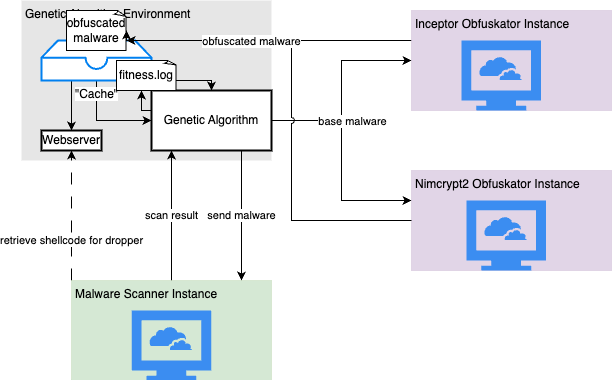
\includegraphics[width=0.85\textwidth]{gfx/Abbildungen/Architektur.drawio.png}
    \caption{Architektur von Obscurus Evolved}
    \label{fig:architecture}
\end{figure}

\subsection{Obfuskatoren}
Um die beiden Modi von PE und RAW gleichermaßen abdecken zu können, wurde sich für eine Auswahl aus Packern entschieden, welche beide Varianten abdecken können und die bereits in der Pipeline integriert waren.
    \subsubsection{Inceptor}
    Inceptor ist ein Tool, welches seinen PE-Input mithilfe von Tools in ein intermittierendes Shellcodeformat verwandelt und auf dieser Ebene dann seine Obfuskationen durchführt. Hierbei erlaubt es Sandboxdeception, Verschlüsselung, verschiedene Generatoren und Encodings...
    \cite{wauters_2024_building}.
    \cite{klezVirus_n.d.} 
    \textbf{ZITATION Prüfen}
    \subsubsection{Nimcrypt2}
    Dieses Tool bietet neben der klassischen Verschlüsselung von Strings und dynamischer Schlüsselgeneration mit AES auch Sandbox Evasion als Möglichkeit an, ebenso wie die Randomisierung von Syscalls der Windows API \cite{icyguider_2022_github}.

    
\subsection{Antivirenscanner}
Windows Defender und Microsoft Defender Enterprise sind die beiden AV Lösungen von Microsoft.  
\textbf{Todo!}

\subsection{Pipeline: Obscurus}
Bei der verwendeten Pipeline namens 'Obscurus' handelt es sich um eine API basierte interne Lösung, die PE und Raw Files nach bestimmten Konfigurationen obfuskiert und die obfuskierte Malware zurück gibt. Neben dem Obfuskationsmodus hat das Tool ebenso noch eine AV-Scan Funktion mit der verschiedene AV Softwaren ein File scannen können und damit erkennen, ob Malware obfuskiert werden konnte.